\documentclass[12pt]{article}

\usepackage{amsmath,amsthm,amsfonts,amssymb,amsxtra}
\usepackage{pgf,tikz}
\usetikzlibrary{arrows}
\renewcommand{\theenumi}{(\alph{enumi})} 
\renewcommand{\labelenumi}{\theenumi}

\pagestyle{empty}
\setlength{\textwidth}{7in}
\setlength{\oddsidemargin}{-0.5in}
\setlength{\topmargin}{-1.0in}
\setlength{\textheight}{9.5in}

\theoremstyle{definition}
\newtheorem{problem}{Problem}

\makeatletter
\newcommand*{\radiobutton}{%
  \@ifstar{\@radiobutton0}{\@radiobutton1}%
}
\newcommand*{\@radiobutton}[1]{%
  \begin{tikzpicture}
    \pgfmathsetlengthmacro\radius{height("X")/2}
    \draw[radius=\radius] circle;
    \ifcase#1 \fill[radius=.6*\radius] circle;\fi
  \end{tikzpicture}%
}
\makeatother

\begin{document}

\noindent{\large\bf MATH 122}\hfill{\large\bf Exam \#3.}\hfill{\large\bf
  Fall 2016}\hfill{\large\bf Page 1/5}\hrule

\bigskip
\begin{center}
  \begin{tabular}{|ll|}
    \hline & \cr
    {\bf Name: } & \makebox[12cm]{\hrulefill}\cr & \cr
    {\bf VIP ID:} & \makebox[12cm]{\hrulefill}\cr & \cr
    \hline
  \end{tabular}
\end{center}
\begin{itemize}
\item Write your name and your VIP ID in the space provided above.
\item The test has five (5) pages, including this one.
\item You must show sufficient work to justify all answers unless
  otherwise stated in the problem.  Correct answers with inconsistent
  work may not be given credit.
\item Credit for each problem is given in parentheses at the right of
  the problem number.
\item No books, or notes may be used on this test.
\item An approved calculator may be used on this test.
\end{itemize}
\hrule

\begin{center}
  \begin{tabular}{|c|c|c|}
    \hline
    &&\cr
    {\large\bf Page} & {\large\bf Max.~points} & {\large\bf Your points} \cr
    &&\cr
    \hline
    &&\cr
    {\Large 2} & \Large 25 & \cr
    &&\cr
    \hline
    &&\cr
    {\Large 3} & \Large 25 & \cr
    &&\cr
    \hline
    &&\cr
    {\Large 4} & \Large 25 & \cr
    &&\cr
    \hline
    &&\cr
    {\Large 5} & \Large 25 & \cr
    &&\cr
    \hline\hline
    &&\cr
    {\large\bf Total} & \Large 100 & \cr
    &&\cr
    \hline
  \end{tabular}
\end{center}
\newpage

%%%%%%%%%%%%%%%%%%%%%%%%%%%%%%%%%%%%% Page 2
\noindent{\large\bf MATH 122}\hfill{\large\bf Exam \#3.}\hfill{\large\bf
  Fall 2016}\hfill{\large\bf Page 2/5}\hrule

\bigskip
\begin{problem}[15 pts]
The function $f(x) = x^4 - 5x^3 + 11x$ has a critical point at $x=1$.  Identify what kind of critical point it is.
\begin{itemize}
\item[\radiobutton] $f(x)$ has a local minimum at $x=1$.
\item[\radiobutton] $f(x)$ has a local maximum at $x=1$.
\item[\radiobutton] $x=1$ is neither maximum, minimum, nor inflection point of $f(x)$.
\item[\radiobutton] $f(x)$ has an inflection point at $x=1$.
\end{itemize}
\end{problem}


\vspace{3cm}
\hrule
\begin{problem}[10 pts]
The function $y=f(x)$ is shown below.  How many inflection points does this function have on the interval shown?
\begin{center}
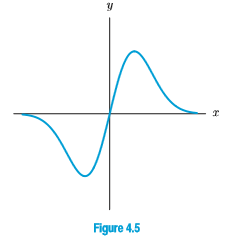
\includegraphics{3graph1.png}
\end{center}
\begin{itemize}
\item[\radiobutton] 0
\item[\radiobutton] 1
\item[\radiobutton] 2
\item[\radiobutton] 3
\end{itemize}
\end{problem}
\newpage

%%%%%%%%%%%%%%%%%%%%%%%%%%%%%%%%%%%%% Page 3
\noindent{\large\bf MATH 122}\hfill{\large\bf Exam \#3.}\hfill{\large\bf
  Fall 2016}\hfill{\large\bf Page 3/5}\hrule

\bigskip
\begin{problem}[10 pts]
Concerning the graph of the function below, which of the following statements is true?
\begin{center}
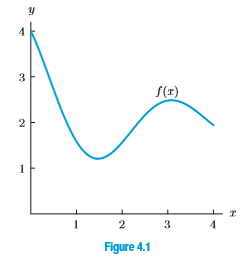
\includegraphics{3graph3}
\end{center}
\begin{itemize}
\item[\radiobutton] The derivative is zero only at one value of $x$, where it is a local minimum.
\item[\radiobutton] The derivative is zero at two values of $x$, both being local maxima.
\item[\radiobutton] The derivative is zero at two values of $x$, one is a local maximum, while the other is a local minimum.
\item[\radiobutton] The derivative is zero at two values of $x$, one is a local maximum on the interval, while the other is neither a local maximum nor a minimum.
\item[\radiobutton] The derivative is zero at two values of $x$, one is a local minimum on the interval, while the other is neither a local maximum nor a minimum.
\end{itemize}
\end{problem}

\hrule
\begin{problem}[15 pts]
Find all local maxima, minima and inflection points of the function $f(x) = 2x^3 + 3x^2-180x+9$.
\end{problem}

\newpage

%%%%%%%%%%%%%%%%%%%%%%%%%%%%%%%%%%%%% Page 4
\noindent{\large\bf MATH 122}\hfill{\large\bf Exam \#3.}\hfill{\large\bf
  Fall 2016}\hfill{\large\bf Page 4/5}\hrule

\bigskip

\begin{problem}[10 pts]
If the graph below is that of $f'(x)$, which of the following statements is true concerning the function $f(x)$?
\begin{center}
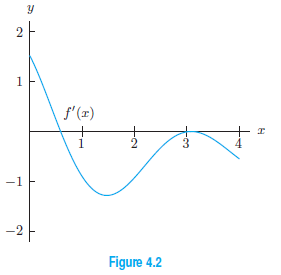
\includegraphics{3graph2}
\end{center}
\begin{itemize}
\item[\radiobutton] The derivative is zero only at one value of $x$, where it is a local minimum.
\item[\radiobutton] The derivative is zero at two values of $x$, both being local maxima.
\item[\radiobutton] The derivative is zero at two values of $x$, one is a local maximum, while the other is a local minimum.
\item[\radiobutton] The derivative is zero at two values of $x$, one is a local maximum on the interval, while the other is neither a local maximum nor a minimum.
\item[\radiobutton] The derivative is zero at two values of $x$, one is a local minimum on the interval, while the other is neither a local maximum nor a minimum.
\end{itemize}
\end{problem}

\hrule
\begin{problem}[15 pts]
Find the global maximum and the global minimum of the function $f(x) = 2x^3 - 9x^2$ over the interval $-1 \leq x \leq 6$.
\end{problem}
\newpage

%%%%%%%%%%%%%%%%%%%%%%%%%%%%%%%%%%%%% Page 5
\noindent{\large\bf MATH 122}\hfill{\large\bf Exam \#3.}\hfill{\large\bf
  Fall 2016}\hfill{\large\bf Page 5/5}\hrule

\bigskip
\begin{problem}[10 pts]
Find the value of constants $a$ and $b$ so that the minimum of the parabola $f(x) = ax^2 -bx +3$ is at $(1,-1)$.

\vspace{7cm}
\end{problem}
\hrule
\begin{problem}[15 pts]
Find the quantity that maximizes profit if the total revenue and total cost (in dollars) are given (resp.) by 
\begin{align*}
R(q) &= 5q - 0.003q^2, \\
C(q) &= 300 + 1.1q,
\end{align*}
where $q$ is quantity and $0 \leq q \leq 1000$ units.  
\end{problem}


\end{document}
